\documentclass[11pt,spanish]{article}

% Paquetes
\usepackage{amstext}
\usepackage{amssymb}
\usepackage{amsmath}
\usepackage{babel}
    \addto\shorthandsspanish{\spanishdeactivate{~<>}}
    \decimalpoint
\usepackage[style=iso]{datetime2}
\usepackage{fancyhdr}
\usepackage{float}
\usepackage[T1]{fontenc}
\usepackage[a4paper]{geometry}
    \geometry{verbose,tmargin=3cm,bmargin=2cm,lmargin=2.5cm,rmargin=2.5cm}
\usepackage{graphicx}
\usepackage{hyperref}
\usepackage[utf8]{inputenc}
\usepackage{lastpage}
\usepackage{mathptmx}
\usepackage{tasks}
\usepackage{units}
\usepackage{siunitx}

% tipo de fuente 
\usepackage{lmodern}

\pagestyle{fancy}
\lfoot{\small DF, FCEyN, UBA}
\cfoot{\tiny Actualizado el {\today} a las {\DTMcurrenttime}}
\rfoot{\small Pág. {\thepage} de \pageref{LastPage}}

\begin{document}

% Título
    \begin{center}
    \textsc{\large Física 2 (Física) -- Cátedra Diego Arbó}
    \par\end{center}{\large \par}
    
    \begin{center}
    \textsc{\large Primer Cuatrimestre de 2025}
    \par\end{center}{\large \par}
    
    \begin{center}
    \textsc{\large Guía 4: Ondas Viajeras}
    \par\end{center}{\large \par}

% Comienzo 
\begin{enumerate}

\section*{Parámetros de ondas viajeras}


% Ejercicio 1

    \item Verifique si las siguientes expresiones matemáticas
    cumplen la ecuación de ondas clásica unidimensional. Grafique
    las funciones dadas.

	\begin{enumerate}
    	\item $\psi(x,t)=Ae^{-\lambda(x-vt)^{2}}$
    	\item $\psi(x,t)=\beta(x+vt)$
    	\item $\psi(x,t)=A\sin\left[k(x-vt)\right]$
    	\item $\psi(x,t)=B\sin^{2}\left(kx-\omega t\right)$
    	\item $\psi(x,t)=C\cos(kx)\sin(\omega t)$
    	\item $\psi(x,t)=De^{i(kx-\omega t)}$
	\end{enumerate}


% Ejercicio 2

    \item Una onda se propaga en una cuerda produciendo una oscilación
    transversal dada por:
    $$\psi(x,t) = \SI{0.1}{\metre} \sen \left( \SI{\pi}{\per\metre} x - \SI{4 \pi}{\per\second} t \right)$$
    Determine:
    \begin{enumerate}
    	\item la amplitud de la onda;
    	\item su frecuencia de oscilación;
    	\item su velocidad de propagación;
    	\item el desplazamiento, velocidad y aceleración del segmento de cuerda
        ubicado en $x = \SI{2}{\metre}$ en el tiempo $ t = \SI{1}{\second}$.
    \end{enumerate}


% Ejercicio 3

    \item Considere una onda tranversal que se propaga a lo largo de la
    dirección $x$, con frecuencia angular $\omega= \SI{10}{\per\second}$ y
    número de onda $k = \SI{100}{\per\metre}$. En $x_1 = \SI{1}{\kilo\metre}$ y
    $t_1 = \SI{1}{\second}$ la fase de la onda es $\phi = \frac{3 \pi}{2}$.

    \begin{enumerate}
    	\item ¿Cuál es la fase en la posición $x_1$ para tiempo $t = 0$?
    	\item Considerando que $\phi(x,t) = k x - \omega t+ \phi_0$, ¿cuánto
        vale $\phi_0$?
    	\item ¿A qué velocidad se propaga la onda?
    	\item ¿Cuánto tiempo tarda un frente de onda para viajar desde $x_1$
        hacia $x_2 = 2 x_1$?
    \end{enumerate}


% Ejercicio 4

    \item Una cuerda de densidad lineal $\mu = \SI{0.005}{\kilo\gram\over\metre}$
    se tensa con una fuerza de \SI{0.25}{\newton}. Un extremo de la cuerda se
    desplaza transversalmente (mediante la aplicación de una fuerza externa),
    siendo la distancia entre los desplazamientos extremos igual a
    \SI{0.4}{\metre}, y el tiempo que tarda en recorrer dicha distancia igual a
    \SI{0.25}{\second}. Encontrar:
    \begin{enumerate}
    	\item La velocidad de la onda generada en la cuerda, su frecuencia y su
        longitud de onda.
    	\item La expresión matemática para el desplazamiento $\psi(x,t)$.
    	\item La energía cinética media por unidad de longitud, para una
        partícula del medio.
    	\item La energía potencial media por unidad de longitud, para la misma
        partícula.
    \end{enumerate}

\section*{Superposición de ondas viajeras}


% Ejercicio 5

    \item Una cuerda de longitud $L = \SI{0.6}{\metre}$, fija en sus dos
    extremos, oscila en uno de sus modos normales, tal como muestra la figura.
    La velocidad de propagación de las ondas en dicha cuerda es
    $v = \SI{80}{\metre\over\second}$. La máxima amplitud pico a pico es
    $\SI{8}{\milli\metre}$.

    \begin{figure}[H]
        \centering{}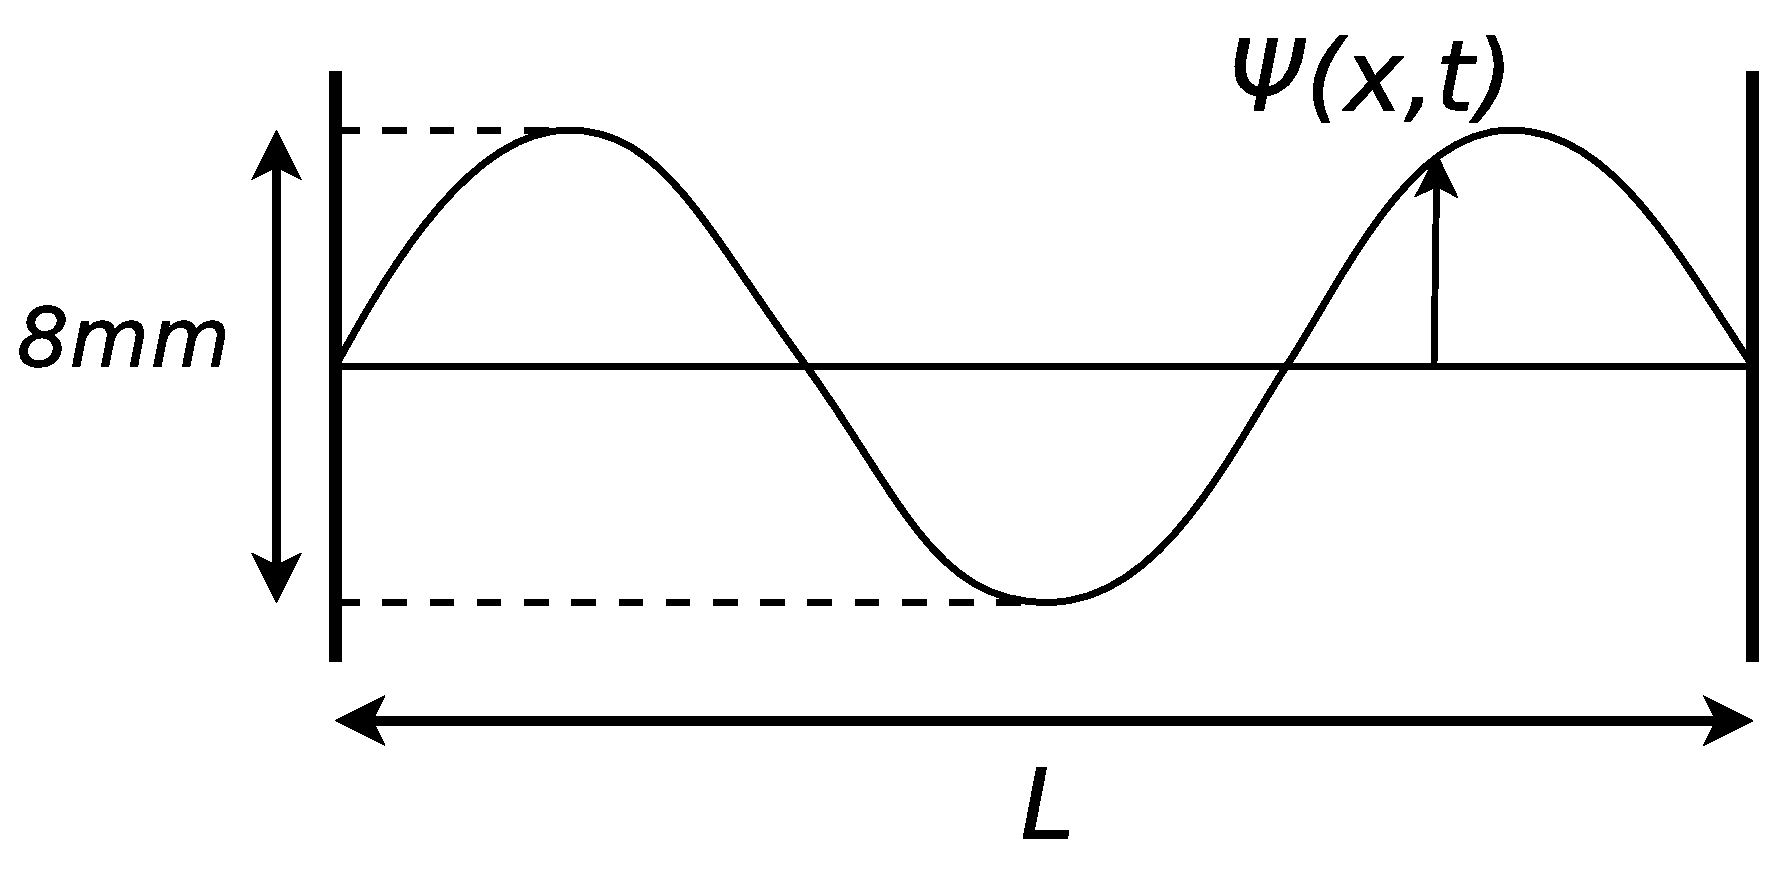
\includegraphics[clip,scale=0.25]{figs/ej1-32}
    \end{figure}
    
    \begin{enumerate}
    	\item Escribir $\psi(x,t)$, sabiendo que $\psi(x,0) = 0\;\forall x$, y
        que $\dot{\psi}(L/2,0) > 0$.
    	\item Hallar ondas viajeras $\psi_\text{der}$ y $\psi_\text{izq}$
        tales que $\psi(x,t)$ sea una combinación lineal de éstas.
    \end{enumerate}

    
% Ejercicio 6
    
    \item Una cuerda de longitud $L = \SI{1}{\metre}$, con un extremo fijo y uno
    libre, oscila en uno de sus modos normales, tal como muestra la figura. La
    velocidad de propagación de las ondas en dicha cuerda es $v=\SI{80}{\metre\over\second}$.
    La máxima amplitud pico a pico es $\SI{8}{\milli\metre}$, siendo
    $\psi(L,0) > 0$.

    \begin{figure}[H]
        \centering{}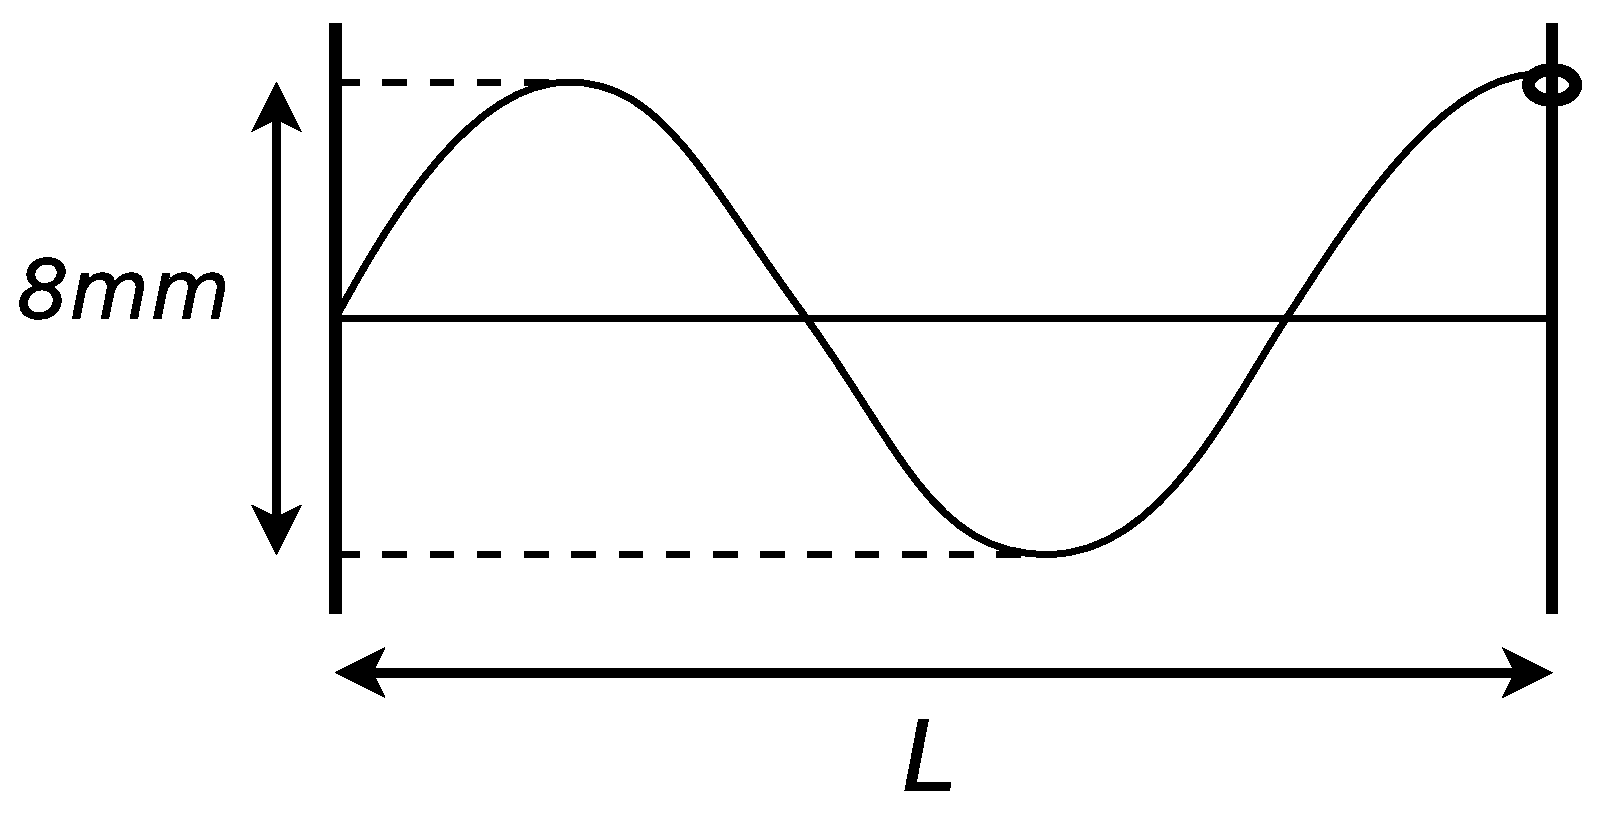
\includegraphics[clip,scale=0.25]{figs/ej1-33}
    \end{figure}
    
    \begin{enumerate}
    	\item Resolver, para esta situación, todo lo pedido en el problema
        anterior. 
    	\item Si ahora la cuerda está oscilando en un modo normal arbitrario $n$,
        con las mismas condiciones dadas arriba, repetir (a) (expresar en
        función de $n$).
    \end{enumerate}

    
\section*{Condiciones iniciales}

\textbf{Comentario:} Los siguientes ejercicios pueden resolverse usando la
solución de D'Alembert para la ecuación de ondas\textsuperscript{\href{https://en.wikipedia.org/wiki/D%27Alembert%27s_formula
}{link}},
o bien aplicando desarrollo de Fourier.

% Ejercicio 7
    
    \item Se tiene una perturbación que se propaga en una cuerda infinita con
    velocidad $v$. Se toman dos ``fotografías'' de la perturbación, a $t=0$ s y
    $t=4$ s:

    \begin{figure}[H]
        \centering{}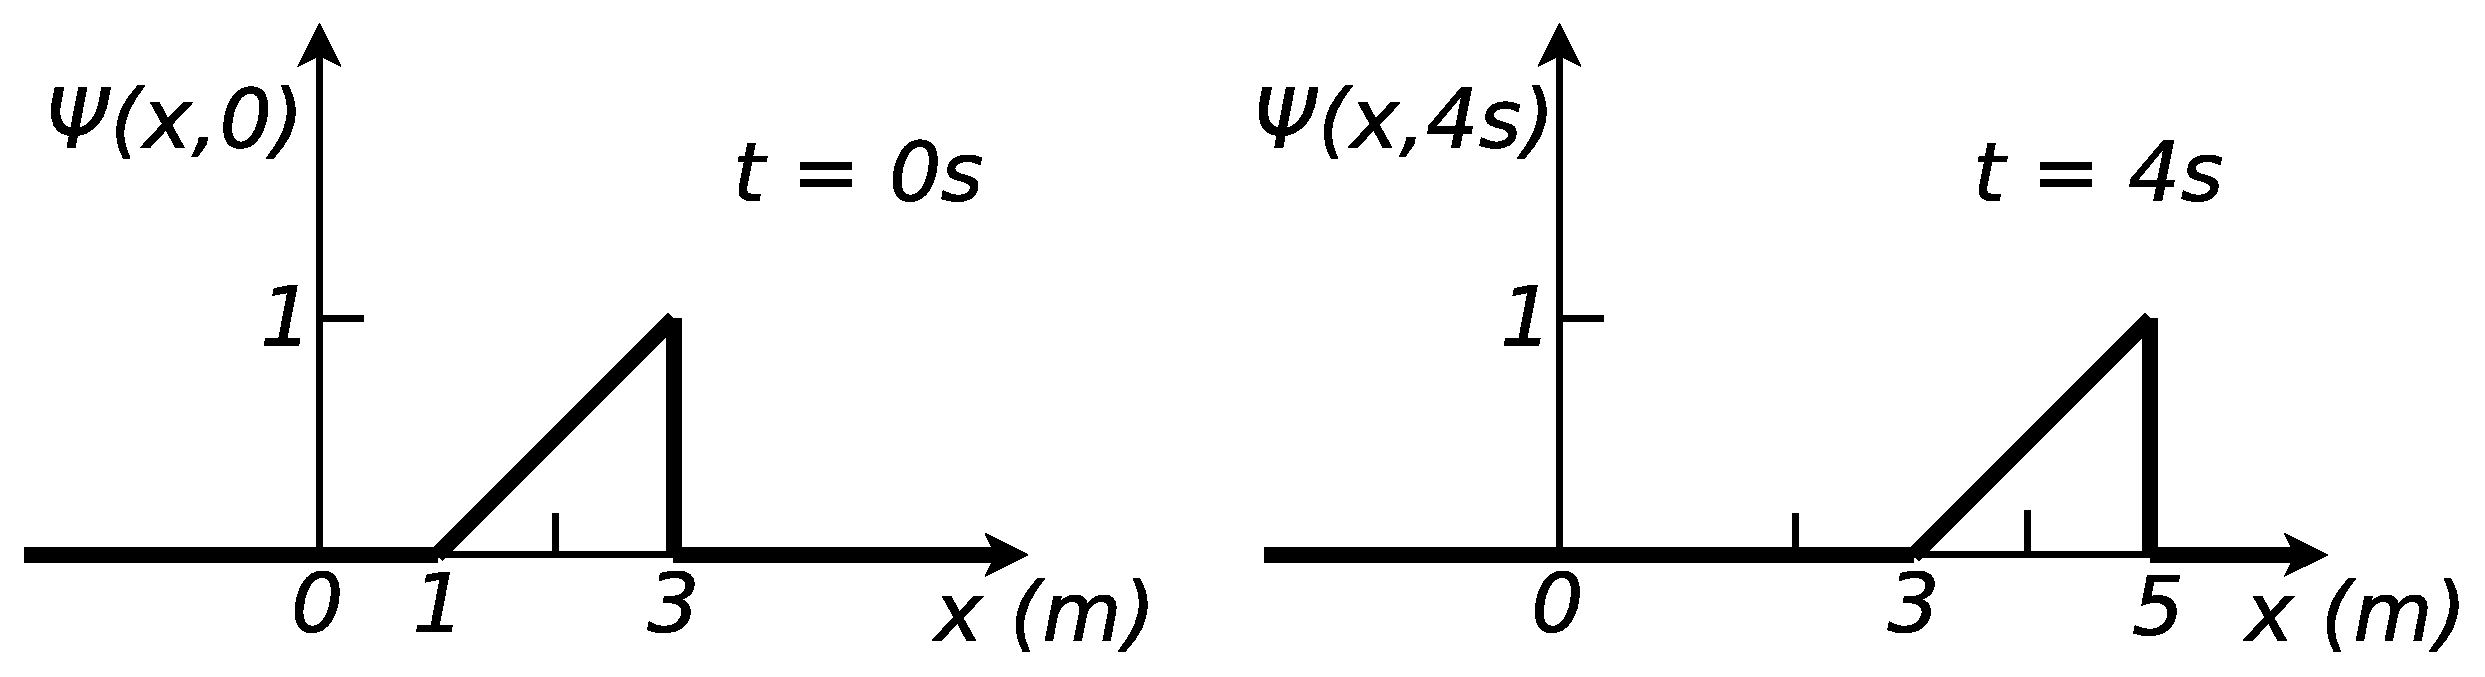
\includegraphics[clip,scale=0.25]{figs/ej2-2}
    \end{figure}

    \begin{enumerate}	
        \item ¿Cuánto vale la velocidad de propagación de la perturbación $v$?.
        \item Halle $\psi(x,t)$ .
        \item Calcule la velocidad transversal.
    \end{enumerate}
    

% Ejercicio 8

    \item Se tiene una cuerda infinita. Se sabe que la velocidad de propagación
    de las ondas en ella es $v=100$ m/s (consideramos que dicha cuerda es un
    medio no dispersivo). A $t=0$ se la deforma de la manera que se indica en la
    figura, y se la suelta desde el reposo.
    
    \begin{figure}[H]
        \centering{}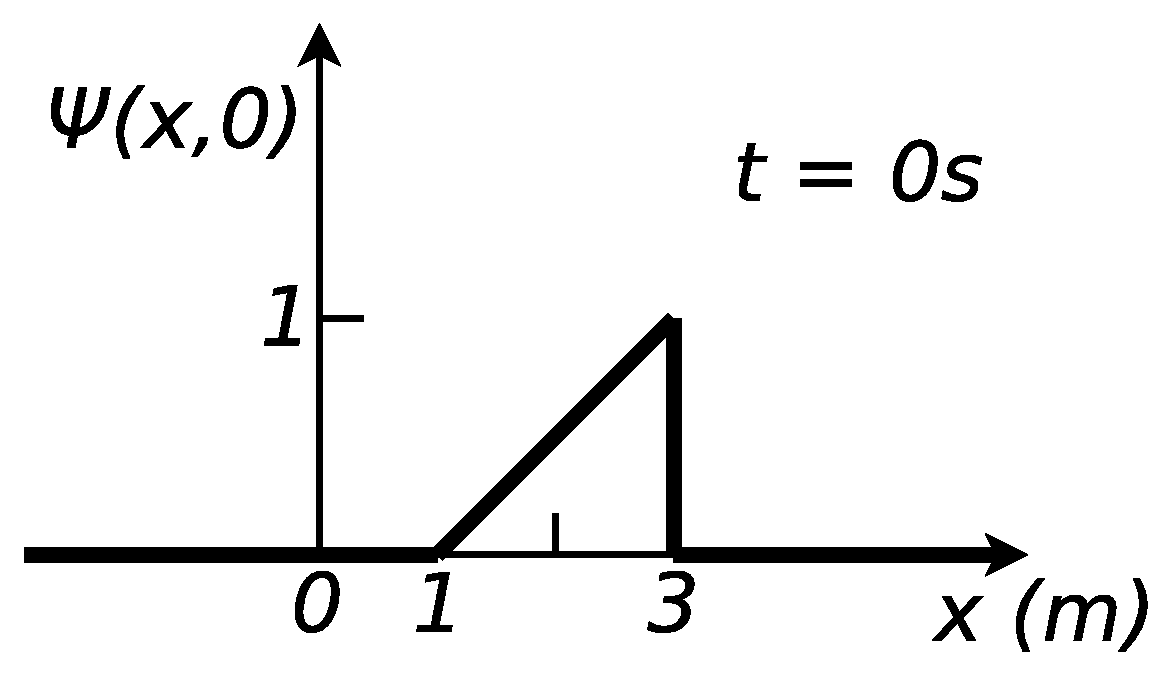
\includegraphics[clip,scale=0.25]{figs/ej2-3}
    \end{figure}

    \begin{enumerate}
        \item Hallar $\psi(x,t)=\psi_{1}(x-vt)+\psi_{2}(x+vt)$. Dar explícitamente
        (en cada intervalo de interés) la expresión de $\psi(x,t)$. 
        \item Comparar esta situación con la del problema anterior. 
    \end{enumerate}

% Ejercicio 9

    \item Se tiene una cuerda homogénea de longitud $L$ y densidad $\mu$, a una
    tensión $T$, con sus dos extremos fijos $(x=0\mbox{ y }x=L)$. A $t=0$ se la
    perturba de forma tal que:

    $$\psi(x,0)=\begin{cases}
        0 & \mbox{si }0<x<a \\
        h\frac{x-a}{L/2-a} & \mbox{si }a<x<L/2 \\
        h\frac{L-a-x}{L/2-a} & \mbox{si }L/2<x<L-a \\
        0 & \mbox{si }L-a<x<L.
    \end{cases}$$

    Se suelta la cuerda desde el reposo; considerar $h\ll L$. 

    \begin{enumerate}
        \item Hallar $\psi(x,t)$ y demostrar que siempre es posible escribir esta
        solución como una superposición de una onda que se propaga hacia la
        derecha y una que se propaga hacia la izquierda.
        \item Hacer un esquema cualitativo del movimiento de la cuerda para los
        instantes $t_{n}=n\frac{L}{8v}$, donde $v$ es la velocidad de propagación
        de las ondas en la cuerda y $n$ es un número natural.
    \end{enumerate}
    
% Ejercicio 10
    
    \item En un gas, a $t=0$, se produce la perturbación indicada en la figura.
    Sabiendo que $\frac{\rho_{1}-\rho_{0}}{\rho_{0}}\ll1$
    y que el sistema parte del reposo (es decir, $\dot\psi(x,0)=0$), calcule
    $\rho(x,t)$. 

    \begin{figure}[H]
        \centering{}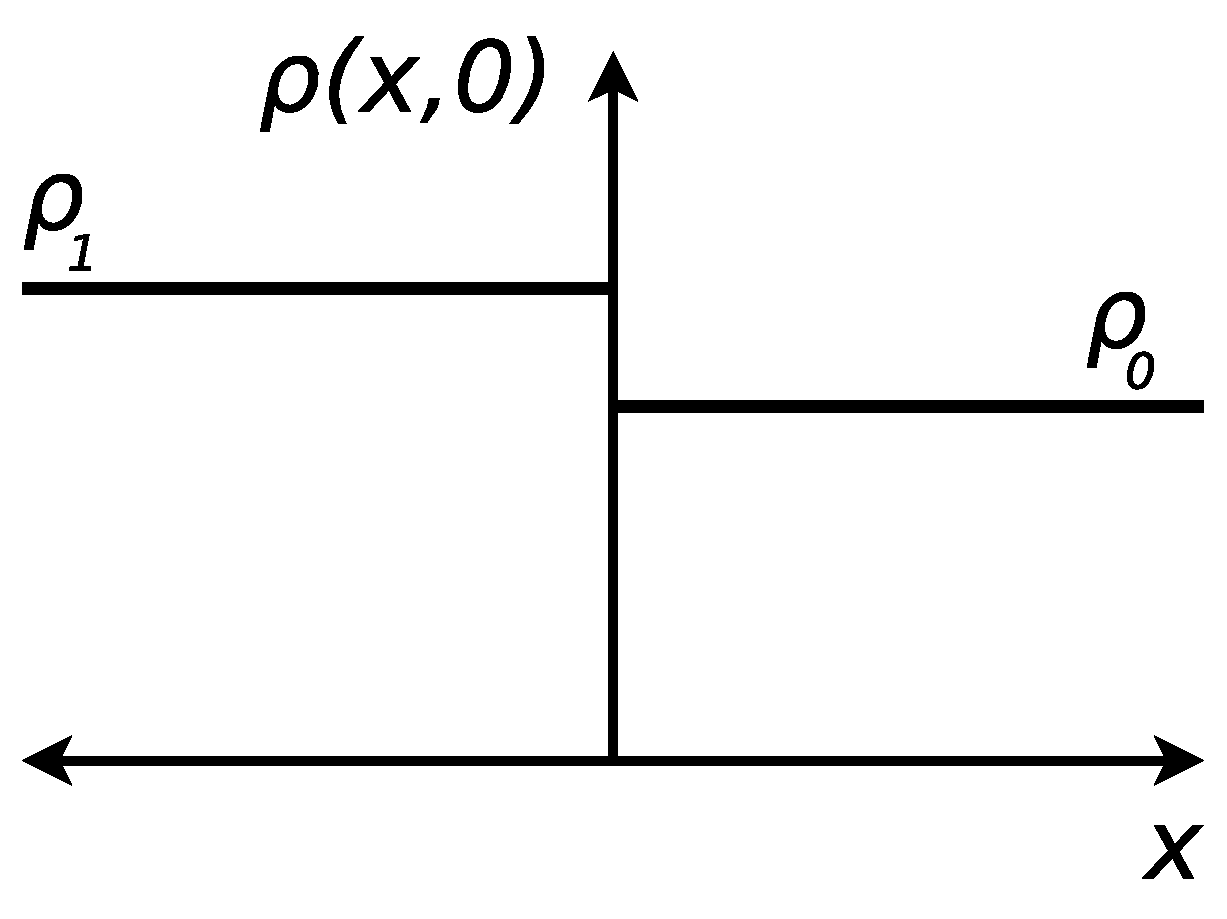
\includegraphics[clip,scale=0.25]{figs/ej2-5}
    \end{figure}

    \textbf{Sugerencia:} Puede comenzar planteando condiciones de contorno
    apropiadas en $x= \pm L$ para luego pedir que $L \to \infty$. ¿Cómo se
    modifica el desarrollo de la condición inicial en una serie de modos
    normales al hacer esto? \textbf{Ayuda:} Tenga en cuenta la relación de
    dispersión.

    \textbf{Datos:} $\rho_{1}$, $\rho_{0}$, $v_\text{s}$ (velocidad de
    propagación de las ondas en el gas, a.k.a., \textit{velocidad del sonido}).

\section*{Fuentes en movimiento (optativos)}

% Ejercicio 11

	\item \textbf{Efecto Doppler:} Una fuente de sonido que emite en una
	frecuencia de 1000 Hz se mueve hacia la derecha a 40 m/s. Un observador,
	que está a la derecha de la fuente, también se mueve hacia la derecha
	a 20 m/s.

	\begin{enumerate}
		\item ¿Cuál será la frecuencia detectada por el observador? El aire se encuentra
		en reposo.
		\item Repita el punto anterior si hay viento hacia la derecha a 20 m/s.
		\item Repita todo lo hecho si el observador se encuentra inicialmente a
		la izquierda de la fuente.
	\end{enumerate}

% Ejercicio 12

	\item \textbf{Ondas de choque:} Un avión a retropropulsión en vuelo horizontal
	a 5000 m de altura pasa sobre un observador con velocidad $2.2$ Mach
	(o sea, $2.2$ veces la velocidad del sonido). Calcular:

	\begin{enumerate}
		\item El ángulo formado por el frente de la onda sonora y la dirección del
		movimiento.
		\item ¿Cuánto tiempo después de haber pasado el avión sobre el observador
		la onda llega a éste?
		\item Si el piloto hace sonar una bocina en el instante en que pasa justo
		sobre el observador, ¿cuánto tiempo después escucha el observador
		ese sonido?
	\end{enumerate}

\end{enumerate}

\end{document}
